\documentclass[german, 12pt, oneside, numbers=noenddot]{scrbook}
\usepackage{geometry}                		
%\usepackage{german}
%\usepackage{ngerman}
\usepackage[german]{babel}
%\usepackage[parfill]{parskip}    			% Activate to begin paragraphs with an empty line rather than an indent
\usepackage{graphicx}						% Use pdf, png, jpg, or epsß with pdflatex; use eps in DVI mode
											% TeX will automatically convert eps --> pdf in pdflatex		

%\usepackage{helvet}						% Kommentar wegnehmen, um in Helvetica zu schreiben
%\renewcommand{\familydefault}{\sfdefault}
%\fontfamily{phv}\selectfont

\usepackage{amssymb}
\usepackage{mathtools} % includes amsmath

\usepackage[utf8]{inputenc}
\usepackage[T1]{fontenc}

\usepackage{lscape}

%\usepackage{arydshln} attention: not compatible with longtable
\usepackage{tabularx}
\usepackage{longtable} % table over multiple pages
\usepackage{multirow}
\usepackage{subfig}
\usepackage{pdfpages}
\usepackage{framed}

\usepackage{forloop}								
\usepackage{listings}
\usepackage{fancyvrb}
\usepackage{color} 
\usepackage{colortbl}
\usepackage{courier}
\usepackage{pifont}

\usepackage[pdftex]{hyperref}
\usepackage{url}

\usepackage{float} % für \begin{figure}[H]
\usepackage{fancyhdr}
\usepackage{lipsum}

\usepackage{multicol} % für mehrspaltige Texte

\usepackage{scrhack}


%	%%%%%%%%%%%%%%%%%%%%%%%%%%%%%%%%%%%%%%%%%%%%%%%%%%%%%%%%
% 	Vermeiden der KOMA Script Fehlermeldung:
%      'Class scrbook Error: undefined old font command `\rm''	
%	%%%%%%%%%%%%%%%%%%%%%%%%%%%%%%%%%%%%%%%%%%%%%%%%%%%%%%%%

\makeatletter
\DeclareOldFontCommand{\rm}{\normalfont\rmfamily}{\mathrm}
\DeclareOldFontCommand{\sf}{\normalfont\sffamily}{\mathsf}
\DeclareOldFontCommand{\tt}{\normalfont\ttfamily}{\mathtt}
\DeclareOldFontCommand{\bf}{\normalfont\bfseries}{\mathbf}
\DeclareOldFontCommand{\it}{\normalfont\itshape}{\mathit}
\DeclareOldFontCommand{\sl}{\normalfont\slshape}{\@nomath\sl}
\DeclareOldFontCommand{\sc}{\normalfont\scshape}{\@nomath\sc}
\makeatother



%	%%%%%%%%%%%%%%%%%%%%%%%%%%%%%%%%%%%%%%%%%%%%%%%%%%%%%%%%
% 	Dokumentabmessungen	
%	%%%%%%%%%%%%%%%%%%%%%%%%%%%%%%%%%%%%%%%%%%%%%%%%%%%%%%%%

\geometry {a4paper, bottom=30mm, left=20mm, right=30mm, top=25mm}


%	%%%%%%%%%%%%%%%%%%%%%%%%%%%%%%%%%%%%%%%%%%%%%%%%%%%%%%%%
% 	Kopfzeile
%	%%%%%%%%%%%%%%%%%%%%%%%%%%%%%%%%%%%%%%%%%%%%%%%%%%%%%%%%

\pagestyle{fancyplain}
\fancyhf{}

% Kopfzeile links: Kapitel rechts: HTL Logo
\lhead{\fancyplain{}{\nouppercase\leftmark}}
\rhead{\fancyplain{}{
\includegraphics[width=2cm]{./media/images/htl_moedling_logo.jpg}}}

%\cfoot{\fancyplain{\thepage}{}}
%\rfoot{\fancyplain{}{\thepage}} %-----------------------


% Auskommentieren der folgenden Zeile setzt das HTL Logo in die
% Mitte der Kopfzeile auf jeder ersten Haupt-Kapitelseite

%\chead{\fancyplain{
\includegraphics[width=1.5cm]{./media/images/htl_moedling_logo.jpg}}{}}


%	%%%%%%%%%%%%%%%%%%%%%%%%%%%%%%%%%%%%%%%%%%%%%%%%%%%%%%%%
% 	Farbdefinitionen	
%	%%%%%%%%%%%%%%%%%%%%%%%%%%%%%%%%%%%%%%%%%%%%%%%%%%%%%%%%

\definecolor{grey}{RGB}{127,127,127}
\definecolor{lightgrey}{RGB}{180,180,180}
\definecolor{dkgreen}{rgb}{0,0.6,0}  
\definecolor{gray}{rgb}{0.5,0.5,0.5} 
\definecolor{mauve}{rgb}{0.58,0,0.82}

\definecolor{cssId}{rgb}		{0,0,0.6 }%{0.75, 0.00, 0.00 }
\definecolor{cssAttribute}{rgb}	{0.58,0,0.82 }%{0.00, 0.00, 0.75 }
\definecolor{cssClass}{rgb}		{0,0,0.6 }%{0.00, 0.75, 0.00 }
\definecolor{cssComment}{rgb}	{0,0.6,0 }%{0.00, 0.75, 0.00 }
\definecolor{cssString}{rgb}	{0.6,0,0 }%{0.00, 0.75, 0.00 }



%	%%%%%%%%%%%%%%%%%%%%%%%%%%%%%%%%%%%%%%%%%%%%%%%%%%%%%%%%
% 	Diverse Befehle		
%	%%%%%%%%%%%%%%%%%%%%%%%%%%%%%%%%%%%%%%%%%%%%%%%%%%%%%%%%

%	Quelltext im Textfluss
\def\inlinecode#1{\texttt{\color{gray}{#1}}}


%	Paragraph mit Zeilenumbruch nachher
\def\htlParagraph#1{\paragraph*{#1}$\;$ \\}

%   Short Version of \today
\newcommand{\leadingzero}[1]{\ifnum #1<10 0\the#1\else\the#1\fi}
\newcommand{\todayshort}{\leadingzero{\day}.\leadingzero{\month}.\the\year}

%	%%%%%%%%%%%%%%%%%%%%%%%%%%%%%%%%%%%%%%%%%%%%%%%%%%%%%%%%
% 	Code Formatierung		
%	%%%%%%%%%%%%%%%%%%%%%%%%%%%%%%%%%%%%%%%%%%%%%%%%%%%%%%%%
\lstset{literate=%
{Ö}{{\"O}}1 
{Ä}{{\"A}}1 
{Ü}{{\"U}}1 
{ß}{{\ss}}2 
{ü}{{\"u}}1 
{ä}{{\"a}}1 
{ö}{{\"o}}1
}
 
\lstset{ % 
%  language=Octave,                			% the language of the code 
 	basicstyle=\ttfamily\footnotesize, 		% the size of the fonts that are used for the code 
	numbers=left,                   		% where to put the line-numbers 
	numberstyle=\tiny\color{gray},  		% the style that is used for the line-numbers 
	stepnumber=1,                   		% the step between two line-numbers. If it's 1, each line  
                                  			% will be numbered 
	numbersep=5pt,                  		% how far the line-numbers are from the code 
	backgroundcolor=\color{white},    	  	% choose the background color. You must add \usepackage{color}
	showspaces=false,               		% show spaces adding particular underscores 
	showstringspaces=false,      	   		% underline spaces within strings
	showtabs=false,                 		% show tabs within strings adding particular underscores
%	frame=single,                   		% adds a frame around the code
	frame=l,
	rulecolor=\color{dkgreen},        		% if not set, the frame-color may be changed on line-breaks within not-black text (e.g. comments (green here))
	tabsize=2,                      		% sets default tabsize to 2 spaces
	captionpos=b,                   		% sets the caption-position to bottom
	breaklines=true,                		% sets automatic line breaking
	breakatwhitespace=false,        		% sets if automatic breaks should only happen at whitespace
%	title=\lstname,                   		% show the filename of files included with \lstinputlisting;
          	                        		% also try caption instead of title
	keywordstyle=\color{blue},          	% keyword style
	commentstyle=\color{dkgreen},       	% comment style
	stringstyle=\color{mauve},    	     	% string literal style
	escapeinside={\%*}{*)},            		% if you want to add LaTeX within your code
	morekeywords={*,...},              		% if you want to add more keywords to the set
	deletekeywords={...}             	 	% if you want to delete keywords from the given language
}

%	%%%%%%%%%%%%%%%%%%%%%%%%%%%%%%%%%%%%%%%%%%%%%%%%%%%%%%%%
% 	CSS		
\lstdefinelanguage{CSS}{
		alsoletter={\\,/,*,:,-,\#,.},
		identifierstyle=\idstyle,
        keywords={accelerator:, azimuth:, background:, background-attachment:, background-color:, background-image:, background-position:, background-position-x:, background-position-y:, background-repeat:, behavior:, border:, border-bottom:, border-bottom-color:, border-bottom-style:, border-bottom-width:, border-collapse:, border-color:, border-left:, border-left-color:, border-left-style:, border-left-width:, border-right:, border-right-color:, border-right-style:, border-right-width:, border-spacing:, border-style:, border-top:, border-top-color:, border-top-style:, border-top-width:, border-width:, bottom   :, caption-side:, clear:, clip:, color:, content:, counter-increment:, counter-reset:, cue:, cue-after:, cue-before:, cursor:, direction:, display:, elevation:, empty-cells :, filter:, float:, font:, font-family:, font-size:, font-size-adjust:, font-stretch:, font-style:, font-variant:, font-weight:, height:, ime-mode:, include-source:, layer-background-color:, layer-background-image:, layout-flow:, layout-grid:, layout-grid-char:, layout-grid-char-spacing:, layout-grid-line:, layout-grid-mode:, layout-grid-type:, left:, letter-spacing:, line-break:, line-height:, list-style:, list-style-image:, list-style-position:, list-style-type:, margin:, margin-bottom:, margin-left:, margin-right:, margin-top:, marker-offset:, marks:, max-height:, max-width:, min-height:, min-width:, -moz-binding:, -moz-border-radius:, -moz-border-radius-topleft:, -moz-border-radius-topright:, -moz-border-radius-bottomright:, -moz-border-radius-bottomleft:, -moz-border-top-colors:, -moz-border-right-colors:, -moz-border-bottom-colors:, -moz-border-left-colors:, -moz-opacity:, -moz-outline:, -moz-outline-color:, -moz-outline-style:, -moz-outline-width:, -moz-user-focus:, -moz-user-input:, -moz-user-modify:, -moz-user-select:, orphans:, outline:, outline-color:, outline-style:, outline-width:, overflow:, overflow-X:, overflow-Y:, padding:, padding-bottom:, padding-left:, padding-right:, padding-top:, page:, page-break-after:, page-break-before:, page-break-inside:, pause:, pause-after:, pause-before:, pitch:, pitch-range:, play-during:, position:, quotes:, -replace:, richness:, right:, ruby-align:, ruby-overhang:, ruby-position:, -set-link-source:, size:, speak:, speak-header:, speak-numeral:, speak-punctuation:, speech-rate:, stress:, scrollbar-arrow-color:, scrollbar-base-color:, scrollbar-dark-shadow-color:, scrollbar-face-color:, scrollbar-highlight-color:, scrollbar-shadow-color:, scrollbar-3d-light-color:, scrollbar-track-color :, table-layout:, text-align:, text-align-last:, text-decoration:, text-indent:, text-justify:, text-overflow:, text-shadow:, text-transform:, text-autospace:, text-kashida-space:, text-underline-position:, top:, unicode-bidi:, -use-link-source:, vertical-align:, visibility:, voice-family:, volume :, white-space:, widows:, width:, word-break:, word-spacing:, word-wrap:, writing-mode},
        keywordstyle=\color{cssAttribute},%\bfseries,
        ndkeywords={@import, @media, @page, @font-face, @charset, @namespace, a, html, body, title, pre, h1, h2, h3, h4, h5, h6, ul, ol, li, p, br, blockquote, dl, dt, dd, div, img, strong, em, cite, tt, i, b, table, tr, td, th, frame, form, option, input, button, nav, section, article, aside, footer, hr, sup, sub, del, ins, small, span},
        ndkeywordstyle=\color{cssId},%,\bfseries,
%        identifierstyle=\color{black},
%        sensitive=false,
%        comment=[l]{//},
        morecomment=[s]{/*}{*/},
        commentstyle=\color{cssComment}\ttfamily,
        stringstyle=\color{cssString}\ttfamily,
        morestring=[b]',
        morestring=[b]"
}

\makeatletter
\newcommand*\idstyle[1]{%
         \expandafter\id@style\the\lst@token{#1}\relax%
 }

 \def\id@style#1#2\relax{%
           	\ifnum\pdfstrcmp{#1}{\#}=0%
                \small\ttfamily\color{cssId} \the\lst@token%
            \else%
		      	\ifnum\pdfstrcmp{#1}{.}=0%
    	            \small\ttfamily\color{cssClass} \the\lst@token%
        		\else%
					\ifnum\pdfstrcmp{#1}{:}=0%
    	            	\small\ttfamily\color{cssAttribute} \the\lst@token%
    	         	\else%
		     	 		%\edef\tempa{\uccode#1}%
              			\edef\tempa{\lccode`#1}%
              			\edef\tempb{`#1}%
              			\ifnum\tempa=\tempb%
                			\small\ttfamily\color{mauve} \the\lst@token%
              			\else%
                 	 		\the\lst@token%
    	         		\fi%
	           		\fi%
	            \fi%
            \fi%
 }
\makeatother



%	%%%%%%%%%%%%%%%%%%%%%%%%%%%%%%%%%%%%%%%%%%%%%%%%%%%%%%%%
% 	JavaScript	
\lstdefinelanguage{JavaScript}{
        keywords={typeof, new, true, false, catch, function, return, null, catch, switch, var, if, in, while, do, else, case, break},
		alsoletter={\{,\}\\,/,*,:,-,\#,.},
 %       keywordstyle=\color{blue}\bfseries,
        ndkeywords={class, export, boolean, throw, implements, import, this},
%        ndkeywordstyle=\color{darkgray}\bfseries,
%        identifierstyle=\color{black},
%        sensitive=false,
        comment=[l]{//},
        morecomment=[s]{/*}{*/},
%        commentstyle=\color{purple}\ttfamily,
%        stringstyle=\color{red}\ttfamily,
        morestring=[b]',
        morestring=[b]"
}



%	%%%%%%%%%%%%%%%%%%%%%%%%%%%%%%%%%%%%%%%%%%%%%%%%%%%%%%%%
% 	TypoScript	
\lstdefinelanguage{TypoScript}{
        keywords={typeof, new, true, false, catch, function, return, null, catch, switch, var, if, in, while, do, else, case, break},
		alsoletter={\{,\}\\,/,*,:,-,\#,.},
 %       keywordstyle=\color{blue}\bfseries,
        ndkeywords={class, export, boolean, throw, implements, import, this},
%        ndkeywordstyle=\color{darkgray}\bfseries,
%        identifierstyle=\color{black},
%        sensitive=false,
        comment=[l]{//},
        morecomment=[s]{/*}{*/},
%        commentstyle=\color{purple}\ttfamily,
%        stringstyle=\color{red}\ttfamily,
        morestring=[b]',
        morestring=[b]"
}
	

\usepackage[onehalfspacing]{setspace}
\usepackage{csquotes}
\usepackage{graphicx}
\usepackage{uarial} % Load uarial package for Arial font

% C#
\usepackage{listings}

% Fußnotenpackage
\usepackage{fancyhdr}
\usepackage{lastpage}

% to_donotes
\usepackage{todonotes}

% highlighting
\usepackage{xcolor, soul}

% maybe use german grammar package 

% ende
% Variables
\def\Betreuer{Hack Niklas}
\def\DPThema{Unity Game Design und Development}

% vl. Variablen für die Autoren 
% \def\Hauptverantwortlicher{Lukas Schachinger}
% \def\Zweitverantwortlicher{Martin Usta}

\newcommand{\newglossaryentryfast}[3]{%
    \newglossaryentry{#1}{%
        name={#2},
        description={#3},
    }
}

\lstdefinelanguage{CSharp}
{
    language=[Sharp]C,
    keywordstyle=\color{blue},
    commentstyle=\color{green!50!black},
    stringstyle=\color{red},
    morekeywords={var,get,set}
}

% Define a new page style 'customfooter' with the footer
\fancypagestyle{customfooter}{
  \fancyfoot[C]{HTBLuVA-Mödling \hfill \authorname \hfill Seite \thepage\ von \pageref{LastPage}}
}

% Command to set the author name for the footer
\newcommand{\setauthorname}[1]{\def\authorname{#1}}

% Default page style without the footer
\pagestyle{empty}

% Better Glossary entries, it will make a footnote + a glossary entry
\newcommand{\bettergls}[2]{%
  \gls{#1}\footnote[#2]{\glsentrydesc{#1}}%
}


\usepackage{glossaries}
\makenoidxglossaries
\newglossaryentryfast{multiplayer}{Multiplayer}{Beschreibt den Videospiel Modus bei dem mehrere Menschen mit oder gegeneinander spielen.}

\newglossaryentryfast{UI}{User Interface}{Beschreibt die Schnittstelle zwischen Mensch und Computer.}

\newglossaryentryfast{singleplayer}{Singleplayer}{Beschreibt den Videospielmodus, bei dem eine einzelne Person das Spiel alleine spielt.}

\newglossaryentryfast{theme}{Theme}{Beschreibt die Gestaltung, den Stil, die Handlung und die Atmosphäre des Spiels.}

\newglossaryentryfast{canvas}{Canvas}{Ein Canvas (Leinwand) ist eine Fläche in einer Grafik- oder Game Engine, auf der Grafiken, Texte oder Benutzeroberflächenlemente gerendert werden können.}

\newglossaryentryfast{gameObject}{Game-Objekt}{Ein Game-Objekt ist eine grundlegende Einheit in einer Game Engine, die verschiedene Komponenten und Eigenschaften haben kann und im Spiel platziert und manipuliert werden kann.}

\newglossaryentryfast{skybox}{Skybox}{Eine Skybox ist ein Grafikelement in einer 3D-Umgebung, das den Eindruck eines fernen Himmels oder einer weit entfernten Umgebung erzeugt.}

\newglossaryentryfast{code-behind}{Code-behind}{Code-behind bezieht sich auf den Programmcode, der hinter Logik oder Funktionalität liegt.}

\newglossaryentryfast{statemachine}{State Machine}{Eine State Machine (Zustandsmaschine) ist ein Konzept in der Softwareentwicklung, das zur Steuerung von Zuständen und Übergängen verwendet wird.}

\newglossaryentryfast{jumprun}{Jump'n'Run}{Jump'n'Run ist ein Videospielgenre, bei dem der Spieler mit Springen und Laufen versuchen muss Hindernisse zu überwinden und Gegner zu besiegen.}

\newglossaryentryfast{collider}{Collider}{Ein Collider ist eine Kollisionskomponente in einer Game Engine, die zur Erkennung von Kollisionen zwischen Game-Objekten verwendet wird.}

\newglossaryentryfast{deathzone}{Deathzone}{Eine Deathzone ist eine Todeszone in der Charakter sozusagen stirbt.}

\newglossaryentryfast{dachRegion}{D-A-CH Region}{Die D-A-CH Region besteht aus Deutschland, Österreich und der Schweiz.}

\newglossaryentryfast{SVoD}{SVod}{Bedeutet Subscription-Video-on-Demand, Video streaming für das die Benutzer ein Monats- oder Jahres Abonnement abschließen.}

\newglossaryentryfast{indie}{Indie}{Indie bedeutet unabhänging. Ein Indie Spiel ist unabhängig von einem Herausgeber wie zum Beispiel \glqq Nintendo\grqq. }

\newglossaryentryfast{void}{Void}{Das Void ist die Dunkelheit unter der Spielwelt. Wenn ein Spieler hineinfällt stirbt dieser oder bekommnt Schaden.}

\newglossaryentryfast{index}{Index}{Index ist eine Stelle in einem Array.}

\newglossaryentryfast{iteriert}{Iteriert}{Iterieren ist der Prozess des durchlaufen einer Sammlung von Daten.}

\newglossaryentryfast{prop}{Prop}{Props interaktive Objekte sein, die vom Spieler genutzt werden können, oder rein ästhetische Elemente, die die Spielwelt bereichern.}

\newglossaryentryfast{npc}{NPC}{ein Non-Playable-Character ist eine vom Computer gesteuerte Spielfigur.}

\newglossaryentryfast{topology}{Topology}{Topology (Topologie) beschreibt in Computerspielen die räumliche Anordnung von Spielobjekten und deren Beziehungen zueinander.}

\newglossaryentryfast{hp}{HP}{HP steht für "Hit Points" (Trefferpunkte). In vielen Videospielen repräsentieren HP die Gesundheit oder Ausdauer eines Charakters.}

\newglossaryentryfast{gameplay}{Gameplay}{Gameplay ist ein entscheidender Aspekt für die Qualität und den Unterhaltungswert eines Spiels.}

\newglossaryentryfast{flow}{Flow}{Flow (Flow-Erlebnis) beschreibt einen Zustand des vertieften und mühelosen Spielens, bei dem der Spieler in einem Videospiel vollständig in die Aufgabe eintaucht.}

\newglossaryentryfast{gamemechaniken}{Gamemechaniken}{Gamemechaniken sind Spielelemente welche man benötigt um das Spiel zu verwenden zum Beispiel Steurung und Fähigkeiten.}

\newglossaryentryfast{platformer}{Platformer}{Ein Platformer (Plattformspiel) ist ein Spielgenre, bei dem die Spielfigur hauptsächlich auf Plattformen springt, klettert oder sich bewegt, um Hindernisse zu überwinden und das Spielziel zu erreichen.} %maybe Platformer ist ein Spielkonzept wo die Spielfigur auf Platformen spring um weiter zu kommen

\newglossaryentryfast{ide}{IDE}{Eine IDE ist eine integrierte Entwicklungsumgebung.}

\newglossaryentryfast{coroutine}{Coroutine}{Coroutinen werden häufig in der Programmierung verwendet, um asynchrone Aufgaben zu behandeln und die Leistung zu verbessern.}

%\glsaddallunused % if glossar is acting up

\usepackage[ natbib=true, style=numeric,sorting=none]{biblatex}
\addbibresource{media/literatur.bib}

%\setlength{\headheight}{23.5071pt}
\setlength{\headheight}{23.7771pt}
\addtolength{\topmargin}{-6.5071pt}

% noindent
\setlength\parindent{0pt}

\begin{document}
\setauthorname{}
\pagestyle{customfooter}


\pagenumbering{arabic}	
		
% !TEX root = ../Vorlage_DA.tex

%	########################################################
% 							Deckblatt
%	########################################################


\titlehead{%
\begin{tabular}{@{}lcr@{}}
\raisebox{-0.5\height}{
\includegraphics[width=0.15\linewidth]{media/images/htl_moedling.png}} &
\begin{minipage}[c]{0.7\linewidth}
\begin{center}
{\bfseries\sffamily\large HÖHERE TECHNISCHE BUNDES - LEHR- UND\\[0.2em]
VERSUCHSANSTALT MÖDLING}\\[1ex]
{\normalsize Höhere Lehranstalt für Elektronik und Technische Informatik\\
Kolleg für Informatik}
{\textcolor{gray}{bzw. Aufbaulehrgang für Informatik}}
\end{center}
\end{minipage} &
\raisebox{-0.5\height}{
\includegraphics[width=0.15\linewidth]{media/images/htl-bildung-mit-zukunft}}
\end{tabular} \\ \\
\rule{1.05\linewidth}{0.4pt}
}

\title{\DPThema}
\subtitle{ {\Large Diplomarbeit}\\[1em]Schulautonomer Schwerpunkt\\ Programmieren und Software Engineering}

\author{\\[1em] 
\emph{ausgeführt im Schuljahr 2022/2023 von:} \\[1em] 
Lukas Schachinger, 6AAIFT\\[1ex] 
Martin Usta, 6AAIFT\\[2em]
\emph{Betreuer:} \\[1em]
 Dipl.-Ing. Niklas Hack
}
\date{\today}

\begin{titlepage}	
\maketitle
\end{titlepage}

\chapter{Eidesstattliche Erklärung}

Ich/Wir erkläre/n an Eides statt, dass ich/wir die vorliegende Diplomarbeit selbstständig und ohne fremde Hilfe verfasst, andere als angegebene Quellen und Hilfsmittel nicht direkt benutzt und die benutzten Quellen wörtlich und inhaltlich entnommenen Stellen als solche erkenntlich gemacht habe/n.
\vspace{3cm}

\begin{tabularx}{\textwidth}{l p{1cm} l p{1cm} X}


Mödling, \todayshort & & Lukas Schachinger & & \hrulefill \\
\emph{Ort, Datum} & & \emph{Verfasser} & & \emph{Unterschrift} \vspace{2cm}\\ 

Mödling, \todayshort & & Martin Usta & & \hrulefill \\
\emph{Ort, Datum} & & \emph{Verfasser} & & \emph{Unterschrift} \vspace{2cm}\\ 

\end{tabularx}

\chapter{Dokumentation}

\renewcommand{\arraystretch}{2} % Anpassen der Zeilenhöhe

\begin{tabular}{|m{0.3\textwidth}|m{0.7\textwidth}|}
\hline
Namen der Verfasser/innen & \\
\hline
Jahrgang & \\
\hline
Thema der Diplomarbeit &  \\
\hline
Kooperationspartner & \\
\hline
\end{tabular}

\vspace{10pt}

\noindent
\begin{tabular}{|m{0.3\textwidth}|m{0.7\textwidth}|}
\hline
Aufgabenstellung & \\
\hline
\end{tabular}

\pagebreak

\noindent
\begin{tabular}{|m{0.3\textwidth}|m{0.7\textwidth}|}
\hline
Realisierung & \\
\hline
\end{tabular}

\vspace{10pt}

\noindent
\begin{tabular}{|m{0.3\textwidth}|m{0.7\textwidth}|}
\hline
Ergebnisse & \\
\hline
\end{tabular}

\pagebreak

\noindent
\begin{tabular}{|m{0.3\textwidth}|m{0.7\textwidth}|}
\hline
Typische Grafik, Foto etc. (mit Erläuterung) & \\
\hline
\end{tabular}

\vspace{10pt}

\noindent
\begin{tabular}{|m{0.3\textwidth}|m{0.7\textwidth}|}
\hline
Teilnahme an Wettbewerben, Auszeichnungen & \\
\hline
\end{tabular}

\vspace{10pt}

\noindent
\begin{tabular}{|m{0.3\textwidth}|m{0.7\textwidth}|}
\hline
Möglichkeiten der Einsichtnahme in die Arbeit & Im Archiv der Abteilung Elektronik und Technische Informatik der HTL Mödling. \\
\hline
\end{tabular}

\vspace{10pt}

\noindent
\begin{tabular}{|m{0.325\textwidth}|m{0.325\textwidth}|m{0.325\textwidth}|}
\hline
Approbation \newline (Datum / Unterschrift) & 
{\tiny Prüfer/Prüferin} \newline \newline \vspace{30pt} & 
{\tiny Direktor/Direktorin} \newline {\tiny Abteilungsvorstand/Abteilungsvorständin} \newline \newline \vspace{30pt} \\
\hline
\end{tabular}%

\pagebreak

%here english ----------------------------------------------------------------

\noindent
\begin{tabular}{|m{0.3\textwidth}|m{0.7\textwidth}|}
\hline
Authors & \\
\hline
Academic Year & \\
\hline
Topic &  \\
\hline
Collaboration Partners & \\
\hline
\end{tabular}

\vspace{10pt}

\noindent
\begin{tabular}{|m{0.3\textwidth}|m{0.7\textwidth}|}
\hline
Assignment & \\
\hline
\end{tabular}

\pagebreak

\noindent
\begin{tabular}{|m{0.3\textwidth}|m{0.7\textwidth}|}
\hline
Implementation & \\
\hline
\end{tabular}

\vspace{10pt}

\noindent
\begin{tabular}{|m{0.3\textwidth}|m{0.7\textwidth}|}
\hline
Results &  \\
\hline
\end{tabular}

\pagebreak

\pagebreak
\noindent
\begin{tabular}{|m{0.3\textwidth}|m{0.7\textwidth}|}
\hline
Typical Graphics, Photos, etc. (with Explanation) & \\
\hline
\end{tabular}


\vspace{10pt}

\noindent
\begin{tabular}{|m{0.3\textwidth}|m{0.7\textwidth}|}
\hline
Participation in Competitions, Awards & \\
\hline
\end{tabular}

\vspace{10pt}

\noindent
\begin{tabular}{|m{0.3\textwidth}|m{0.7\textwidth}|}
\hline
Accessibility of \newline Diploma Thesis & Stored in the archive of the secondary technical college of Moedling, department of electronics and computer engineering \\
\hline
\end{tabular}

\vspace{10pt}

\noindent
\begin{tabular}{|m{0.325\textwidth}|m{0.325\textwidth}|m{0.325\textwidth}|}
\hline
Approval (Date / Signature) &
 {\tiny Examiner \newline \newline} \vspace{30pt} &
  {\tiny Head of College / Department \newline \newline} \vspace{30pt} \\
\hline
\end{tabular}

	
\tableofcontents

\pagebreak
\setauthorname{Lukas Schachinger \& Martin Usta}
\chapter{Pflichtenheft}
\section{Zielbestimmung}


\subsection{Musskriterien}



\pagebreak

\subsection{Wunschkriterien}


\subsection{Abgrenzungskriterien}


\section{Projektumfeldanalyse}

\chapter{Projektplan}
\section{Gesamtprojektplan}

\newcolumntype{C}[1]{>{\centering\arraybackslash}p{#1}}

\noindent
\begin{tabular}{|C{3cm}|C{3cm}|C{3cm}|C{3cm}|C{3cm}|}
\hline
\multicolumn{5}{|c|}{\cellcolor{green!20} Projekt} \\
\hline
\cellcolor{green!20}Analyse des Umfelds/Projektplanung & & & & \\
\hline
& \cellcolor{green!20} Erstellung des Grundgerüsts für den Prototyp & & & \\
\hline
& & \cellcolor{green!20} Fertigstellung der UI & & \\
\hline
& & & \cellcolor{green!20} Fertigstellung des Prototyps & \\
\hline
& & & & \cellcolor{green!20} Diplomarbeit Fertigstellen \\
\hline
\end{tabular}


\vspace{10pt}

\noindent
\begin{tabular}{|C{2.43cm}|C{2.43cm}|C{2.43cm}|C{2.43cm}|C{2.43cm}|C{2.43cm}|C{2.43cm}|}
    Projektstart & Meilenstein 1 Ende & Meilenstein 2 Ende & Meilenstein 3 Ende & Meilenstein 4 Ende & Meilenstein 5 Ende \\
    01.09.2022 & 30.11.2022 & 18.12.2022 & 28.02.2023 & 31.05.2023 & 01.09.2023 \\
\end{tabular}


\pagebreak

\section{Meilensteine}
\subsection{Analyse des Umfelds / Projektplanung}
Zeitraum: 01.09.2022 – 30.11.2022\\\\
Tätigkeiten:
\begin{itemize}
    \item Recherche der Programme
    \item Recherche der Spiel-Engines
    \item Umfeldanalyse Unity gegen Unreal Engine
    \item Umfeldanalyse der unterschiedlichen Modellierprogramme
    \item Kategorisierung der Projektschwerpunkte
    \item Zeiteinteilung der Projektschwerpunkte
    \item Einrichtung des Projektmanagementtools 
\end{itemize}

\todo{Weiter Meilensteine}

\pagebreak

\section{Analyse des Umfelds / Projektplanung}
\begin{tabular}{|m{0.7\textwidth}|m{0.3\textwidth}|}
\hline
\multicolumn{2}{|c|}{\textbf{Analyse des Umfelds / Projektplanung von 01.09.2022 bis 30.11.2022}} \\
\hline
Tätigkeit & Hauptverantwortliche/r \\
\hline
Recherche der Programme & Schachinger, Usta \\
\hline
Recherche der Spiel-Engines & Schachinger \\
\hline
Umfeldanalyse Unity gegen Unreal Engine & Schachinger \\
\hline
Umfeldanalyse der unterschiedlichen Modellierprogramme & Usta \\
\hline
Kategorisierung der Projektschwerpunkte & Schachinger, Usta \\
\hline
Zeiteinteilung der Projektschwerpunkte & Schachinger, Usta \\
\hline
Einrichtung des Projektmanagementtools & Usta \\
\hline
\end{tabular}

\todo{Weiter Meilensteine}

\pagebreak

\section{Arbeitsplan}
\subsection{Planung}
\subsubsection{Pflichtenheft}
\begin{tabular}{|m{0.3\textwidth}|m{0.7\textwidth}|}
\hline
\textbf{Name} & \textbf{Tätigkeit / Verantwortung} \\
\hline
Schachinger Lukas & Autor, hauptverantwortlich \\
\hline
Usta Martin & Autor \\
\hline
\end{tabular}

\subsubsection{Systemspezifikation}
\begin{tabular}{|m{0.3\textwidth}|m{0.7\textwidth}|}
\hline
\textbf{Name} & \textbf{Tätigkeit / Verantwortung} \\
\hline
Schachinger Lukas & Autor, hauptverantwortlich \\
\hline
Usta Martin & Autor \\
\hline
\end{tabular}

\subsubsection{Projekt – und Arbeitsplan}
\begin{tabular}{|m{0.3\textwidth}|m{0.7\textwidth}|}
\hline
\textbf{Name} & \textbf{Tätigkeit / Verantwortung} \\
\hline
Schachinger Lukas & Autor, hauptverantwortlich \\
\hline
Usta Martin & Autor \\
\hline
\end{tabular}

\chapter{Kurzfassung}



\chapter{Abstract}


\setauthorname{Lukas Schachinger}
\chapter{Einleitung}


\section{Problemstellung}

\pagebreak

\chapter{Umfeldanalysen}
\section{Umfeldanalyse von ...}
In der folgenden Umfeldanalyse werden drei ... miteinander verglichen. Anhand der Auswahlkriterien: \textit{Programmierung, Relevanz und Marktanteil} und \textit{Dokumentation und Lektüre} wird entschieden, welche ... für die Diplomarbeit am besten geeignet ist.

\subsection{Allgemeine Auswahlkriterien}
\begin{itemize}
  \item \textbf{Relevanz und Marktanteil:}\\\\ In dem Vergleichspunkt Relevanz und Marktanteil wird gezeigt, für welche Arten von Spielen die Game Engine benutzt wurde. Es soll außerdem dargestellt werden, wie stark die Game Engine auf dem Markt vertreten ist.
  \item \textbf{Programmierung:}\\\\ Die Programmierung beschreibt, wie und mit welchen Programmiersprachen in der Game Engine umgegangen wird. Es wird unterschieden zwischen dem Schreiben von Spielskripten und dem visuellen Skripten.
  \item \textbf{Dokumentation und Lektüre:}\\\\ Der Vergleichspunkt Dokumentation und Lektüre beschreibt, wie viele und welche Art von Dokumentationen verfügbar sind. 
\end{itemize}

\pagebreak

\subsection{Vergleichspunkt1}
\subsubsection{Relevanz und Marktanteil}

\subsubsection{Programmierung}

\subsubsection{Dokumentation und Lektüre (Community)}

\subsection{Entscheidung}

\pagebreak


\chapter{chapter}
\setauthorname{autor 1}

\section{section}
\subsection{subsection}
\subsubsection{subsubsection}

Unity (auch bekannt als Unity3D) ist eine Game Engine und \bettergls{ide}{1} zum kreieren von Interaktionsmedien, meißt Video Spielen. \Cite[][A history of the unity game engine]{haas2014history} \\


\bettergls{hp}{2} wird in der Fußnote genauer beschrieben und ist eingetragen in dem Glossar.


\begin{figure}[H]
    \centering
    
\includegraphics[width=0.2\linewidth]{chapters/00/images/Csharp.png}
    \caption{Das Logo von der Programmiersprache C\#.}
    \label{temp1}
\end{figure}


% C#
\begin{lstlisting}[language=CSharp,caption={Hello World},label=code:hello_world]
    static void Main(string[] args)
    {
        System.Console.WriteLine("Hello World!");
    }
\end{lstlisting}  

\pagebreak
\section{seite 2 mit anderem autor}
\setauthorname{autor 2}

\begin{figure}[h]
    \centering
    \begin{minipage}[b]{0.4\textwidth}
      \centering
      
\includegraphics[width=0.3\textwidth]{chapters/00/images/Csharp.png}
      \caption{Nochmal das Logo von der Programmiersprache C\#.}
      \label{temp2}
    \end{minipage}
    \hfill
    \begin{minipage}[b]{0.4\textwidth}
        \centering
        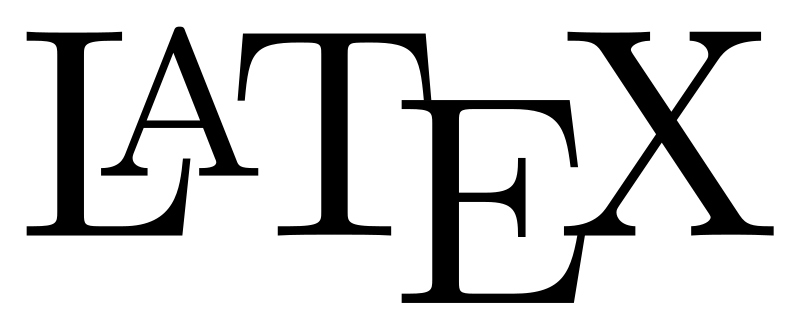
\includegraphics[width=0.3\textwidth]{chapters/00/images/latex.png}
        \caption{Hier das Latex Logo}
        \label{temp3}
    \end{minipage}
    \label{}
\end{figure}

\section{Auflistung}

\begin{itemize}
    \item item 1 
    \item item 2 
    \item item 3
\end{itemize}

%\input{./chapters/14/14_unity.tex}
%\input{./chapters/13/13_blender.tex}

%\input{./chapters/11/11_spieleperformance.tex}
%\input{./chapters/12/12_spieldesign.tex}
%\input{./chapters/15/15_storyandtheme.tex}

%\input{./chapters/03/03_UserInterface.tex}
%\input{./chapters/04/PrototypEntwicklung.tex}

%\input{./chapters/05/ScriptsDescription.tex}

\pagebreak
\setauthorname{Lukas Schachinger}

\chapter{Fazit}
Das letzte Kapitel dieser Diplomarbeit widmet sich der Frage: \glqq \textbf{Wie entwickelt man ein Computerspiel von Grund auf} \grqq. Während der Arbeit haben wir uns umfassend damit befasst, worauf es bei der Spielentwicklung ankommt. \\

Angefangen hat es mit der Überlegung des grundlegenden Konzeptes des Spiels. Zudem befassten wir uns mit dem Game Designs, der Storytelling-Elemente und der Spielmechaniken. Diese Teile sind das Grundgerüst jedes Spiels und legen den Grundstein für die gesamte Entwicklung.\\

Die technische Umsetzung ist der nächstwichtigste Punkt bei der Kreation eines Spieles. Zuerst muss man sich mit der Auswahl der richtigen Game Engine und Grafikdesigntools auseinandersetzen. Erst dann kann man sich mit der eigentlichen Entwicklung beschäftigen.\\

Wie in dem Kapitel \verb+Entwicklung des Prototyps+ beschrieben kann es passieren, dass mehere Versionen des Spieles erstellt werden muss. Dies ist ein großer Teil bei der Entwicklung eines Spieles. Diese Angehensweise ist hilfreich bei dem Testen oder der Verfeinerung der verschiedenen Aspekte des Spieles. In unserem Beispiel haben wir mehrere Versionen des ersten Levels erstellt um kleine Verbesserungen einzubauen oder bekannte Fehler auszubessern.\\

Zusammenfassend lässt sich sagen, dass die Spielentwicklung sowohl kreativ als auch technisch anspruchsvoll ist. Mit Hingabe und der Bereitschaft zum Lernen können Entwickler wie wir beeindruckende Spielerlebnisse erschaffen. Die sich stetig verändernde Branche eröffnet zudem Möglichkeiten, eigene Visionen zu verwirklichen und sich mit den neuesten Techniken zu beschäftigen.

\newpage
\appendix
\setauthorname{}

\newpage
\printnoidxglossary[sort=standard]

\addcontentsline{toc}{chapter}{List of Figures}
\listoffigures

\addcontentsline{toc}{chapter}{Listings}
\lstlistoflistings

\addcontentsline{toc}{chapter}{Bibliography}
\printbibliography

\chapter{Anhang}
\renewcommand{\arraystretch}{1}
\thispagestyle{empty}
\section{Begleitprotokolle}
\markboth{Begleitprotokolle}{Begleitprotokolle}
\newgeometry{bottom=10mm, left=20mm, right=30mm, top=30mm}

\pagebreak

\subsection{Begleitprotokoll von ...} \todo{Name ausfüllen}

\subsubsection{Stundenzahl nach Meilensteinen}

\begin{tabular}{|m{0.3\textwidth}|m{0.6\textwidth}|m{0.1\textwidth}|}
    \hline
    \cellcolor{gray!10} Datum & \cellcolor{gray!10} Meilenstein & \cellcolor{gray!10} Zeit in Stunden \\
    \hline
    9/2022 - 11/2022 & Analyse des Umfelds Projektplanung & 69 \\
    \hline
    11/2022 - 12/2022 & Erstellung des Grundgerüsts für den Prototyp & 69 \\
    \hline
    12/2022 - 02/2023 & Fertigstellung des UI & 69 \\
    \hline
    02/2023 - 05/2023 & Fertigstellung des Prototyps & 69 \\
    \hline
    05/2023 - 09/2023 & Diplomarbeit fertigstellen & 69 \\ 
    \hline
    \multicolumn{2}{|c|}{\cellcolor{gray!30}Gesamtdauer} & 69 \\
    \hline
\end{tabular}

\noindent

\vspace{40pt}

\subsubsection{Stundenerfassung}

\begin{tabular}{|m{0.3\textwidth}|m{0.6\textwidth}|m{0.1\textwidth}|}
    \hline
    \cellcolor{gray!10} Zeitraum & \cellcolor{gray!10} Tätigkeiten & \cellcolor{gray!10} Zeit in Stunden \\
    \hline
    9/2022 - 10/2022 & \hl{Beispiel: } Planen... & 69 \\
    \hline
    \multicolumn{2}{|c|}{\cellcolor{gray!30}Gesamtdauer} & 69 \\
    \hline
\end{tabular}

\pagebreak
% Begleitprotokoll zweite Person
\thispagestyle{empty}
\section{Betreuungsprotokolle}
\markboth{Betreuungsprotokolle}{Betreuungsprotokolle}
\newgeometry{bottom=10mm, left=20mm, right=30mm, top=30mm}
% 111111111111111111111111111111111111111111111111111111111111111111111111111

\pagebreak

\noindent
\begin{tabular}{|m{0.2\textwidth}|m{0.6\textwidth}|m{0.2\textwidth}|}
\hline
\raisebox{-0.5\height}{
\includegraphics[width=1\linewidth]{media/images/htl-bildung-mit-zukunft.png}} 
&
\begin{center}
{\bfseries\sffamily\small HÖHERE TECHNISCHE BUNDES-LEHR- UND VERSUCHSANSTALT MÖDLING}\\[1ex]
{\small Höhere Lehranstalt für Elektronik und Technische Informatik\\
Kolleg für Informatik}
{\textcolor{gray}{bzw. Aufbaulehrgang für Informatik}}
\end{center} & 
\begin{center}
    {Reife- und Diplomprüfung}
\end{center} \\
\hline
\end{tabular}
    

\vspace*{20pt}
\subsection*{Betreuungsprotokoll zur Diplomarbeit \hfill lfd. Nr.: 1}
\vspace*{10pt}

\begin{tabular}{m{0.4\textwidth} m{0.5\textwidth}}
\textbf{Themenstellung:} & \DPThema \\
\textbf{Kandidaten/Kandidatinnen:} & Schachinger Lukas, Usta Martin \\ \\
\textbf{Jahrgang:} & 2000/01 \\
\textbf{Betreuer/in:} & \Betreuer \\
\textbf{Ort:} & Mödling \\
\textbf{Datum:} & 01.01.2000\\
\textbf{Zeit:} & 11:11 \\
\end{tabular}

\subsubsection*{Besprechungsinhalt:}
\begin{tabular}{|m{0.2\textwidth}|m{0.8\textwidth}|}
\hline
Name & Notiz \\
\hline
Usta, Schachinger & Anfang der Planung, Planung der Meilensteine, Einarbeitung des nächsten Meilensteins, Einrichten von DevOps Anfang der Umfeldanalyse \\
\hline
Usta & Aufgliederung der Meilensteine in Arbeitspackete,
Zuteilung der Arbeitspackete
Anfang der Umfeldanalyse von Designprogrammen\\
\hline
Schachinger & Aufgliederung der Meilensteine in Arbeitspackete, 
Zuteilung der Arbeitspakete
Anfang der Umfeldanalyse von Game Engines\\
\hline
\end{tabular}

\subsubsection*{Aufgaben:}
\begin{tabular}{|m{0.2\textwidth}|m{0.6\textwidth}|m{0.2\textwidth}|}
\hline
Name & Notiz & zu erledigen bis \\
\hline
Usta & Fertigstellen der Umfeldanalysen 
Analyse von Designprogramm ZBrush & 12.12.2022 \\
\hline
Schachinger & Fertigstellen der Umfeldanalysen
Analyse von den Game Engines: Unreal, GoDot & 12.12.2022 \\
\hline
\end{tabular}

%nächste Betreuungsprotokolle...
% 222222222222222222222222222222222222222222222222222222222222222222222222222

\end{document}